\documentclass[aspectratio=169]{beamer}
\usetheme{Madrid}
\usepackage[utf8]{inputenc}
\usepackage[T1]{fontenc}
\usepackage{tikz}
\usepackage{amssymb}
\usepackage{graphicx}
\setbeamertemplate{navigation symbols}{}
\setbeamercolor{title}{fg=white,bg=blue!70!cyan}
\setbeamercolor{frametitle}{fg=white,bg=blue!70!cyan}
\setbeamercolor{block title}{bg=blue!70!cyan!20,fg=black}
\setbeamercolor{block body}{bg=blue!70!cyan!8,fg=black}
\setbeamercolor{item}{fg=blue!70!cyan}
\setbeamercolor{itemize item}{fg=blue!70!cyan}
\setbeamertemplate{itemize item}[triangle]

\title{G3 — Decisions}
\subtitle{Touching? Score > 10? Out of bounds?}
\author{ByteForge --- Grade 7 --- Game Maker}
\date{}

\begin{document}

\begin{frame}
    \titlepage
\end{frame}

\begin{frame}{Today's Plan}
    \begin{itemize}
        \item Traffic Light
        \item Big or Small
        \item Danger Zone
        \item[$\bigstar$] BOSS --- Dodge at the Edges
    \end{itemize}
\end{frame}

\begin{frame}{IF/ELSE — choosing between paths}
    \large
    \begin{itemize}
        \item An IF only runs when a condition is true. Chaining IF/ELSE IF/ELSE picks between three outcomes
        \item Only one branch ever runs.
    \end{itemize}

    \begin{center}
    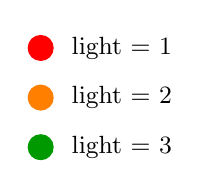
\begin{tikzpicture}[scale=0.9]

        \filldraw[red] (0,0) circle (5pt);
        \filldraw[orange] (0,-0.7) circle (5pt);
        \filldraw[green!60!black] (0,-1.4) circle (5pt);
        \node[right] at (0.3,0) {\small light = 1};
        \node[right] at (0.3,-0.7) {\small light = 2};
        \node[right] at (0.3,-1.4) {\small light = 3};
    \end{tikzpicture}
    \end{center}
\end{frame}


\begin{frame}{Comparisons — greater than, not just equal}
    \large
    \begin{itemize}
        \item "Bigger than 50" covers a whole RANGE. Deciding exactly where a boundary sits is a real, common source of bugs ("off-by-one" errors).
    \end{itemize}
\end{frame}


\begin{frame}{Combining a variable, IF, and drawing}
    \large
    \begin{itemize}
        \item Comparing a changing value against a fixed threshold
        \item The exact pattern you'll build on properly in G6, Collision \& Physics.
    \end{itemize}
\end{frame}


\begin{frame}{BOSS — multiple IFs, one per key}
    \large
    \begin{itemize}
        \item Each arrow key needs its OWN if
        \item Checking every single frame is what makes movement feel continuous, not jumpy.
    \end{itemize}
\end{frame}

\begin{frame}{Real-World Examples}
    \large
    \begin{itemize}
        \item A real traffic light's three states (red/amber/green) is literally an if/else-if/else chain in the controller software
        \item Same three-way branch this chapter teaches. Minecraft redstone comparators/repeaters build these same IF-style circuits entirely out of blocks, no typed code at all.
    \end{itemize}
\end{frame}


\begin{frame}{Image}
    \begin{center}
    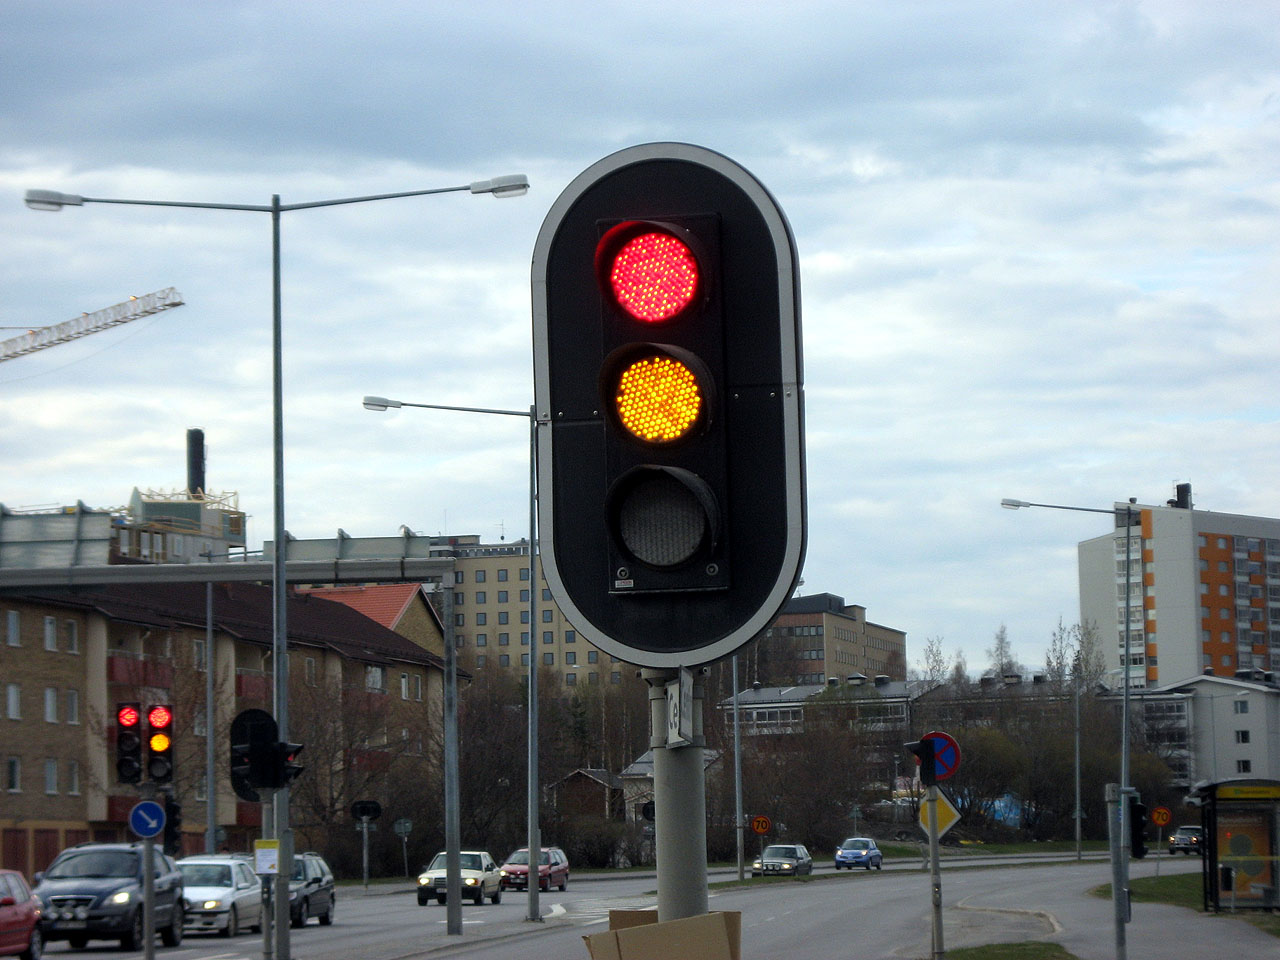
\includegraphics[width=0.5\textwidth]{images/traffic.jpg}

    \large A real three-way branch --- red, amber, green --- running on if/else logic.

    \small LED traffic lights, public domain (PD-self), via Wikimedia Commons
    \end{center}
\end{frame}

\begin{frame}{Let Them Discover}
    \Large
    Find a real rule with a fuzzy boundary (is a "tall" person over 180cm? over 175cm?). Where would YOU draw the line, and would someone exactly on that line be included or not? This is exactly the off-by-one problem in code.
\end{frame}

\begin{frame}{Your Turn}
    \Large
    Open the student map, find \textbf{G3 — Decisions}, and work through it
    hands-on --- everything you just saw, they now do themselves.
\end{frame}

\end{document}
